% short summary/

% TODO: check out MG02 for more details for this section!!!

% TODO: some algebraic background

\section{Notation}
In the following, we denote vectors by bold lower-case letters $\mathbf{v}$ and matrices by bold upper-case letters $\mathbf{M}$. We interchangeably use matrix notation and sets of column vectors $\left[\mathbf{v}_1 \cdots \mathbf{v}_n\right] = \left\{\mathbf{v}_1, \dots, \mathbf{v}_n\right\}$. Unless specified otherwise, by $\| \cdot \|$ or simply \textit{norm} we refer to the Euclidean norm. By $[n]$ we denote the set $\{1, \dots, n\}$ for $n\in \mathbb{N} \setminus \{0\}$. We denote the logarithm base $2$ by $\log$ and the natural logarithm with base $e$ by $\ln$. In order to avoid confusion, throughout this work, we let $\sigma$ denote the standard deviation, and set $s =\sigma \sqrt{2 \pi}$ and $\alpha = \frac{s}{q} = \frac{\sqrt{2\pi} \sigma}{q}$ for other commonly used Gaussian parameters.
% TODO: anything else? Inner product, negation in ring
% add alpha, s, sigma here?

\section{Norms}\label{sec:norms}
We can define the standard $\ell_p$-norms on the vector space $\mathbb{R}^n$. In this work, we will also consider rings and modules (see \cref{sec:ring-module}) and require a way to bound the length of ring and module elements. Let $\mathcal{R}_q=\mathbb{Z}_q[X]/\langle X^n + 1 \rangle$ be a quotient ring as defined in \cite{BDLOP18} and $f \in \mathcal{R}_q$ with $f = \sum_i f_i X^i$. Following \cite{BDLOP18}, we define the norms
\begin{equation}
    \begin{aligned}
        \ell_1 : \| f \|_1           & = \sum_i |f_i|,                                         \\
        \ell_2 : \| f \|_2           & = \sqrt{\sum_i |f_i|^2},                                \\
        \ell_p : \| f \|_p           & = \left(\sum_i |f_i|^p\right)^{\frac{1}{p}} \text{ and} \\
        \ell_\infty : \| f \|_\infty & = \max_i |f_i|.
    \end{aligned}
\end{equation}
For standard vector spaces, the definitions are essentially equivalent to the above, except that $f$ is a vector in $\mathbb{R}^n$ or, in our case, $\mathbb{Z}^n$ with coefficients $f_i$. For a module element $\mathbf{f} \in \mathcal{R}_q^d$, we can simply view $\mathbf{f}$ as a $n\cdot d$-dimensional vector.

\section{Lattices}
%%%%%%%%%%%%%%%%%%%%%%%%%%%%%%%%%%%%%%%%%%%%%%%%%%%
%%%%%%%%%%%%%%%%%%%%%%%%%%%%%%%%%%%%%%%%%%%%%
% TODO: write more intro?
We now present the mathematical definition of lattices and related tools that we will use later on. Most of the background theory is based on material from \cite{MG02} with some adaptions.

A \textit{lattice} $\Lambda$ is a discrete additive subgroup of the vector space $\mathbb{R}^m$. Every lattice can be defined by a basis $\mathbf{B}$ of $n$ linearly independent basis vectors $\mathbf{b}_1, \ldots, \mathbf{b}_n \in \mathbb{R}^m$ with $m\geq n$. A lattice is then the set of all integer linear combinations of the basis vectors in $\mathbf{B}$. \cref{fig:lattice-a} shows a lattice with basis vectors $\mathbf{b}_1 = (0, 1)^\intercal$ and $\mathbf{b}_2 = (2, 1)^\intercal$.

\begin{definition}[Lattice]
    Given a basis $\mathbf{B} = \left[\mathbf{b}_1, \ldots, \mathbf{b}_n\right] \in \mathbb{R}^{m\times n}$, we call $\Lambda$ a lattice generated by the column vectors of $\mathbf{B}$ if
    \begin{equation}
        \Lambda(\mathbf{B}) = \left\{ \mathbf{x} \in \mathbb{R}^m \;\middle\vert\ \; \exists c_1, \ldots, c_n \in \mathbb{Z} : \mathbf{x} = \sum_{i=1}^n c_i \mathbf{b}_i \right\}.
    \end{equation}
\end{definition}

% TODO: make plot
We call $n$ the \textit{rank} of the lattice. A lattice has full rank if the $n=m$. The basis of a lattice $\mathbf{B}$ is not unique. The two example lattices in \cref{fig:lattice} are identical, but have different bases. If $\mathbf{B}$ is a basis of a lattice $\Lambda$, then for any unimodular matrix $\mathbf{U}\in \mathbb{Z}^{n\times n}$ with determinant $\pm 1$, the basis $\mathbf{B}\cdot \mathbf{U}$ is also a basis of $\Lambda$. In cryptographic applications, we usually begin with a lattice basis $\mathbf{B}$ with long basis vectors that are not very orthogonal to each other. For example, the problem of finding a short vector (SVP or SVP$_\gamma$, see \cref{def:svp}) in $\Lambda(\mathbf{B})$ turns out to be very difficult. If we can somehow find a ``nicer'' basis for $\Lambda(\mathbf{B})$ with shorter and more orthogonal basis vectors, finding a solution becomes a lot easier. We can improve the quality of a basis or ``reduce'' a basis in such a way by means of lattice basis reduction. The basis in \cref{fig:lattice-b} is ideal, i.e., it cannot be further reduced, whereas the basis in \cref{fig:lattice-a} can be reduced. In this particular case, the reduction is quite trivial. We can simply compute $\mathbf{b}'_2 = \mathbf{b}_2 - \mathbf{b}_1$ and take $\{\mathbf{b}_1, \mathbf{b}'_2\}$ as our new basis. But more to that later.
\begin{figure}
    \begin{subfigure}{0.5\textwidth}
        \centering
        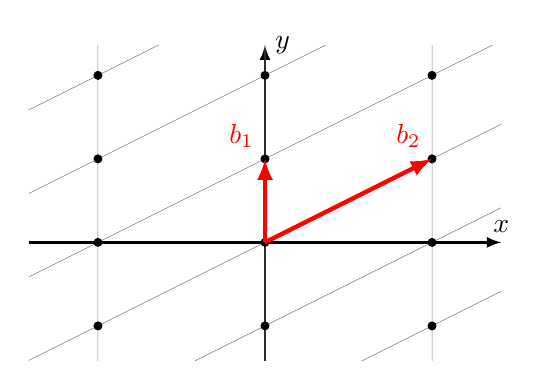
\begin{tikzpicture}[line/.style={>=latex}]
            \coordinate (Origin)   at (0,0);
            \coordinate (XAxisMin) at (-3,0);
            \coordinate (XAxisMax) at (3,0);
            \coordinate (YAxisMin) at (0,-1.5);
            \coordinate (YAxisMax) at (0,2.5);
            \draw [thick, black,-latex] (XAxisMin) -- (XAxisMax) node [above] {$x$};
            \draw [thick, black,-latex] (YAxisMin) -- (YAxisMax) node [right] {$y$};

            \clip (-3,-1.5) rectangle (3, 2.5);
            \pgftransformcm{1.41421356}{0.70710678}{0}{0.7071}{\pgfpoint{0cm}{0cm}}
            \coordinate (Bone) at (0,1.5);
            \coordinate (Btwo) at (1.5,0);
            \draw[style=help lines] (-14,-14) grid[step=1.5cm] (14,14);
            \foreach \x in {-7.5,-6.75,...,7}{
                    \foreach \y in {-7.5,-6.75,...,7}{
                            \node[draw,circle,inner sep=1pt,fill] at (2*\x,2*\y) {};
                        }
                }
            \draw [ultra thick,-latex,red] (Origin)
            -- (Bone) node [above left] {$b_1$};
            \draw [ultra thick,-latex,red] (Origin)
            -- (Btwo) node [above left] {$b_2$};
        \end{tikzpicture}
        \caption{Lattice with basis $\mathbf{b}_1 = (0, 1)^\intercal,\; \mathbf{b}_2 = (2, 1)^\intercal$}
        \label{fig:lattice-a}
    \end{subfigure}
    \begin{subfigure}{0.5\textwidth}
        \centering
        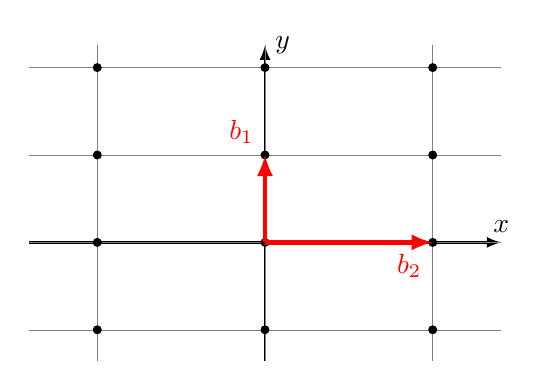
\begin{tikzpicture}[line/.style={>=latex}]
            \coordinate (Origin)   at (0,0);
            \coordinate (XAxisMin) at (-3,0);
            \coordinate (XAxisMax) at (3,0);
            \coordinate (YAxisMin) at (0,-1.5);
            \coordinate (YAxisMax) at (0,2.5);
            \draw [thick, black,-latex] (XAxisMin) -- (XAxisMax) node [above ] {$x$};
            \draw [thick, black,-latex] (YAxisMin) -- (YAxisMax) node [right] {$y$};

            \clip (-3,-1.5) rectangle (3, 2.5);
            \pgftransformcm{1.42}{0}{0}{0.74}{\pgfpoint{0cm}{0cm}}
            \coordinate (Bone) at (0,1.5);
            \coordinate (Btwo) at (1.5,0);
            \draw[style=help lines] (-14,-14) grid[step=1.5cm] (14,14);
            \foreach \x in {-7.5,-6.75,...,7}{
                    \foreach \y in {-7.5,-6.75,...,7}{
                            \node[draw,circle,inner sep=1pt,fill] at (2*\x,2*\y) {};
                        }
                }
            \draw [ultra thick,-latex,red] (Origin)
            -- (Bone) node [above left] {$b_1$};
            \draw [ultra thick,-latex,red] (Origin)
            -- (Btwo) node [below left] {$b_2$};
        \end{tikzpicture}
        \caption{Lattice with basis $\mathbf{b}_1 = (0, 1)^\intercal,\; \mathbf{b}_2 = (2, 0)^\intercal$}
        \label{fig:lattice-b}
    \end{subfigure}
    \caption{Lattice Examples}\label{fig:lattice}
\end{figure}

% TODO: do we need cosets???

Similar to a quotient ring $\mathbb{Z}/q\mathbb{Z}$ of integers modulo some positive integer $q$ with cosets $c + q\mathbb{Z}$, we can define the quotient group $\mathbb{R}^m/\Lambda$ with \textit{cosets}
\begin{equation}
    \mathbf{c} + \Lambda = \{\mathbf{c} + \mathbf{v} \mid \mathbf{v}\in \Lambda\}
\end{equation}
where $\mathbf{c} \in \mathbb{R}^m$ \cite{Pei16}. % TODO: maybe add plot

An important concept is the \textit{fundamental domain} of a lattice. The fundamental domain is a subset of $\mathbb{R}^m$ that contains exactly one representative of every coset of $\mathbb{R}^m/\Lambda$. The most commonly considered fundamental domain of a lattice with basis $\mathbf{B}$ is the (shifted) \textit{fundamental parallelepiped}
\begin{equation} \label{eq:fundamental-parallelepiped}
    \mathcal{P}_{\frac{1}{2}}(\mathbf{B}) = \mathbf{B} \cdot \left[ - \frac{1}{2}, \frac{1}{2}\right)^n = \left\{ \mathbf{x} \in \mathbb{R}^m \;\middle|\; \mathbf{x} = \sum_{i=1}^n c_i \mathbf{b}_i, \; c_i \in  \left[ - \frac{1}{2}, \frac{1}{2}\right) \right\}
\end{equation}
Another region that is often used is the \textit{Voronoi region} $\mathcal{V}$ \cite{GJS15} and is defined as
\begin{equation}\label{eq:voronoi-region}
    \mathcal{V} = \left\{ \mathbf{x} \in \mathbb{R}^n \mid \forall \mathbf{y} \in \Lambda : \| \mathbf{x} \| \leq \| \mathbf{x} - \mathbf{y} \| \right\}.
\end{equation}
% every coset has representative  % c - B * \left\lfloor^{-1} \cdot c\right\rceil
% TODO: first define [0, 1)
% intuition: collection of all points that can be written as By where y in [0, 1)^n
% TODO: maybe add plot

The $n$-dimensional volume of the fundamental parallelepiped of a lattice $\Lambda(\mathbf{B})$ is equivalent to the \textit{determinant} of the lattice $\text{det}(\Lambda(\mathbf{B})) = \sqrt{\text{det}\left(\mathbf{B}^\intercal \mathbf{B}\right)}$. For a full-ranked lattice, the determinant becomes $\det(\Lambda(\mathbf{B})) = |\det(\mathbf{B})|$. The determinant is independent from the used basis, which can be easily verified by looking at $\text{det}(\Lambda(\mathbf{U}\mathbf{B}))$.

The \textit{minimum distance} $\lambda_1(\Lambda)$ of a lattice is the length of its shortest nonzero vector
\begin{equation}
    \lambda_1(\Lambda) = \min_{v \in \Lambda \setminus \{0\}}\|\mathbf{v}\|.
\end{equation}
Furthermore, we can define \textit{$i$th successive minima} $\lambda_i(\Lambda)$ by considering an $m$-dimensional ball $\mathcal{B}(\mathbf{0}, r)$ with increasing radius $r \in \mathbb{R}$ and center $\mathbf{0} \in \mathbb{R}^m$ at the origin of $\Lambda$. Then,  $\lambda_i(\Lambda)$ is the smallest radius $r$ such that the ball $\mathcal{B}(\mathbf{0}, r)$ contains exactly $i$ linearly independent lattice vectors. Note that an optimally reduced basis with basis vectors $\mathbf{b}_1 \leq \mathbf{b}_2 \cdots \leq \mathbf{b}_n$ satisfies $\lambda_i(\Lambda) = \|\mathbf{b}_i\|$ for all $i\in [n]$.


In general, it is hard to determine the exact values of $\lambda_i(\Lambda(\mathbf{B}))$ for a given basis $\mathbf{B}$. \textit{Minkowski's theorem} states that $\lambda_1(\Lambda) \leq \sqrt{n} \cdot (\det(\Lambda))^{\frac{1}{n}}$ given that $\Lambda$ has rank $n$.
The \textit{Gaussian heuristic} is commonly used to estimate the minimum distance $\lambda_1$ of a lattice $\Lambda$ given the determinant $\det{\Lambda}$:
\begin{equation}\label{eq:gaussian-heuristic}
    \lambda_1(\Lambda) \approx \frac{\Gamma(1 + n/2)^{1/n}}{\sqrt{\pi}} \det(\Lambda)^{1/n}
\end{equation}
By applying Stirling's formula to estimate the value of the $\Gamma$-function as described in \cite{Gop16}, we can simply the estimate to
\begin{equation}\label{eq:simplified-gaussian-heuristic}
    \lambda_1(\Lambda) \approx \sqrt{\frac{n}{2\pi e}} \det(\Lambda)^{1/n}
\end{equation}

% TODO: dual lattice
The dual $\Lambda^{\perp}$ of a lattice $\Lambda(\mathbf{B})$ is defined as the set of vectors $\mathbf{y}$ in the span of $\mathbf{B}$, such that the inner product $\langle \mathbf{y}, \mathbf{v} \rangle$  is an integer for all $\mathbf{v} \in \Lambda(\mathbf{B})$. The basis of the dual of a lattice with basis $\mathbf{B}$ is given by $\mathbf{B'} = \mathbf{B} (\mathbf{B}^\intercal \mathbf{B})^{-1}$.

In cryptography, we are mainly interested in modular integer (or $q$-ary) lattices. A $q$-ary lattice is a lattice $\Lambda_q$ such that $q\mathbb{Z}^m \subseteq	\Lambda \subseteq	\mathbb{Z}^m$ given $q \in \mathbb{N}\setminus \{0\}$. This means that a vector $\mathbf{x} \in \mathbb{Z}^m$ is in $\Lambda$ if and only if $\mathbf{x} \text{ mod } q$ also is in $\Lambda$.

We now look at two important ways of specifying a $q$-ary lattice given a matrix $\mathbf{A} \in \mathbb{Z}_q^{n\times m}$ \cite{BBGS19}.
\begin{equation}\label{eq:lwe-lattice}
    \Lambda_q(\mathbf{A}^\intercal) = \left\{ \mathbf{v} \in \mathbb{Z}^m \mid \exists \mathbf{y} \in \mathbb{Z}^n : \mathbf{v} = \mathbf{A}^\intercal \mathbf{y} \mod q \right\}
\end{equation}
$\Lambda_q(\mathbf{A}^\intercal)$ is commonly referred to as the \textit{(primal) LWE lattice}, since finding a short vector in $\Lambda_q(\mathbf{A}^\intercal)$ corresponds to solving LWE. The second, referred to as the \textit{(dual) SIS lattice}, is given by
\begin{equation}\label{eq:sis-lattice}
    \Lambda_q^\perp(\mathbf{A}) = \left\{ \mathbf{v} \in \mathbb{Z}^m \mid  \mathbf{A}\mathbf{v} = \mathbf{0} \mod q \right\}.
\end{equation}
Finding a short vector in $\Lambda_q^\perp(\mathbf{A})$ corresponds to solving the Short Integer Solution problem.

% TODO: find basis of $\Lambda_q(\mathbf{A})$ \cite{AFG13}

In many scenarios, it is convenient to have an explicit formula that describes the relationship between the determinant of the above two lattices and the dimensions of $\mathbf{A}$. For $q$ prime and $m$ sufficiently larger than $n$, we have that the rank of $\mathbf{A}$ is $n$, since the rows of $\mathbf{A}$ are linearly independent with high probability. As a result, the lattice $\Lambda_q(\mathbf{A}^\intercal)$ has $q^n$ points in $\mathbb{Z}_q^m$.
Consider the fundamental domain $D = \mathcal{P}_{1/2}(\Lambda_q(\mathbf{A}^\intercal))$ and the fact that $(\Lambda_q(\mathbf{A}^\intercal) \text{ mod } q) + (D \text{ mod } q) = \mathbb{R}^m/q\mathbb{R}^m$ is a partition \cite{volume-lattice}. The volume of $\mathbb{R}^m/q\mathbb{R}^m$ is given by $q^m =|(\Lambda_q(\mathbf{A}^\intercal) \text{ mod } q)||D \text{ mod } q|$ and thus
\begin{equation}\label{eq:det-MR}
    \text{det}(\Lambda_q(\mathbf{A}^\intercal)) = |D \text{ mod } q| = \frac{q^m}{|(\Lambda_q(\mathbf{A}^\intercal) \text{ mod } q)|} = \frac{q^{m}}{q^{n}} = q^{m-n}.
\end{equation}
Furthermore, we know that the dual lattice  $\Lambda_q^\perp(\mathbf{A})$ has $q^{m-n}$ points in $\mathbb{Z}_q^m$ as the dimension of the kernel of $\mathbf{A}$ is $m-n$. Analogously, we obtain
\begin{equation}\label{eq:det-MR-dual}
    \text{det}(\Lambda_q(\mathbf{A}^\intercal)^{\perp}) = |D \text{ mod } q| = \frac{q^m}{|(\Lambda_q(\mathbf{A}^\intercal) \text{ mod } q)|} = \frac{q^{m}}{q^{m-n}} = q^n.
\end{equation}


Another useful tool it the \textit{Gram-Schmidt orthogonalization} \label{sec:gram-schmidt}. Given a basis $\mathbf{B} = \left[\mathbf{b}_1 \cdots \mathbf{b}_n\right] \in \mathbb{Z}_q^{m\times n}$, we write $\pi_{\text{span}(\mathbf{B})}(\mathbf{t})$ for the projection of a vector $\mathbf{t}$ onto the span of the vectors in $\mathbf{B}$.
% or, more formally,
% \begin{equation}
%   \pi_{\text{span}(\mathbf{B})}(\mathbf{t}) = \mathbf{B}(\mathbf{B}^\perp \mathbf{B})^{-1}\mathbf{B}^\intercal \cdot \mathbf{t}
% \end{equation}
Define $\tilde{\mathbf{b}}_i$ as follows: $\tilde{\mathbf{b}}_1 = \mathbf{b}_1$. For $i \in \{2, \ldots, n\}$, let $\tilde{\mathbf{b}}_i$ be the component of $\mathbf{b}_i$ that is orthogonal to the span of $\left\{\mathbf{b}_1, \ldots, \mathbf{b}_{i-1}\right\}$. In other words,
\begin{equation}
    \tilde{\mathbf{b}}_i = \mathbf{b}_i - \pi_{\text{span}(\mathbf{b}_1, \ldots, \mathbf{b}_{i-1})}(\mathbf{b}_i).
\end{equation} % TODO: define span?
Then,  $\tilde{\mathbf{B}} = \left[\tilde{\mathbf{b}}_1 \cdots \tilde{\mathbf{b}}_n\right]$ is called the Gram-Schmidt orthogonalization of the basis $\mathbf{B}$. We define the Gram-Schmidt coefficients as follows:
\begin{equation}
    \mu_{i, j} = \frac{\left\langle \tilde{\mathbf{b}}_j, \mathbf{b}_i\right\rangle}{\left\langle \tilde{\mathbf{b}}_j, \tilde{\mathbf{b}}_j\right\rangle}
\end{equation}

% TODO Also check out algorithm from AGVW17

We define $\text{dist}(\mathbf{t}, \Lambda(\mathbf{B}))$, where $\Lambda(\mathbf{B}) \subset \mathbb{R}^m$, as the \textit{distance} of a vector $\mathbf{t} \in \mathbb{R}^m$ to the closest lattice vector $\mathbf{v} \in \Lambda(\mathbf{B})$, i.e., $\text{dist}(\mathbf{t}, \Lambda(\mathbf{B})) = \min_{\mathbf{v} \in \Lambda(\mathbf{B})}\|\mathbf{t} -  \mathbf{v}\|$.



% * smoothing lemma



\subsection{Lattice Problems}\label{sec:lattice-problems}
In the previous section, we already mentioned the Shortest Vector Problem or short SVP. In this section, we want to briefly list several lattice problems that are used to show the hardness of LWE and SIS.

\begin{definition}[SVP$_\gamma$] \label{def:svp}
    Given a basis $\mathbf{B}$ of a lattice $\Lambda$, the (approximate) Shortest Vector Problem (SVP$_\gamma$) is the problem of finding a short lattice vector $v\in \Lambda$ such that $0 < \| v \| \leq \gamma \lambda_1(\Lambda)$.
\end{definition}

The corresponding decision version is the \textsc{GapSVP}$_\gamma$ problem, in which we are asked to decide whether $\lambda_1(\Lambda) \leq 1$ or $\lambda_1(\Lambda) \geq \gamma$ given a basis $\mathbf{B}$ of $\Lambda$. If neither is the case, any answer is accepted. In an alternative version of \textsc{GapSVP}$_\gamma$, we have to decide between $\lambda_1(\Lambda) \leq d$ and $\lambda_1(\Lambda) \geq \gamma d$ for some positive real number $d$ \cite{LM09}.

\begin{definition}[SIVP$_\gamma$] \label{def:sivp}
    Given a basis $\mathbf{B}$ of a lattice $\Lambda$ of rank $n$, the (approximate) Shortest Independent Vector Problem (SIVP) is the problem of finding $n$ linearly independent lattice vectors $\mathbf{v}_1, \ldots, \mathbf{v}_n \in \Lambda$ such that $\|\mathbf{v}_i\| \leq \gamma \cdot \lambda_n(\Lambda)$ for all $i \in \{1, \ldots, n\}$.
\end{definition}

Both \textsc{GapSVP}$_\gamma$ and \textsc{SIVP}$_\gamma$ are NP-hard for any constant approximation factor $\gamma$ \cite{Khot05,BS99}. % in all $\ell_p$-norms 
% NP hard for any constant $\gamma$ % Kho04, HR07 see LM09
% fastest algorithm for $1\leq \gamma \leq \text{poly}(n)$ has runtime complexity of $2^{O(n)}$
% In \cref{ch:algorithms}, we will look at some selected algorithms that rely on reductions to the following problems.

% \begin{definition}[CVP$_\gamma$] \label{def:gamma-CVP}
%   Given a basis $\mathbf{B}$ of a lattice $\Lambda \subset \mathbb{R}^m$ and a target vector $\mathbf{t}\in\mathbb{R}^m$, the (approximate)  Closest Vector Problem (CVP$_\gamma$) is the problem of finding a lattice vector $\mathbf{v} \in \Lambda$ with $\|\mathbf{t} - \mathbf{v}\| < \gamma \min_{\mathbf{v}' \in \Lambda} \|\mathbf{v}' - \mathbf{v}\|$.
% \end{definition}
% NP hard in any $\ell_p$-norm for approximation factor $\gamma=1$ \cite{vEB81}


% TODO: add some kind of discussion, e.g. see 1.2 in LM09 or better overview from bootcamp

% * ideal lattice (do I need that?)

% * ...?

% * eher die Sachen für LWE/SIS als die Sachen für Algorithmen (analog Vorlesung), evtl.

% Intuition für die anderen Sachen...



\section{Discrete Gaussian Distribution}

% - Gaussian, def, component-wise, trafo to bound % TODO: GPV08, or LS15

% * definition:
Oftentimes in lattice cryptography, we work with samples or vectors drawn from a discrete uniform or Gaussian distribution. We can define a discrete Gaussian distribution as follows:
\begin{definition}[Discrete Gaussian Distribution \cite{GJS15}]
    The discrete Gaussian distribution $D_{\Lambda, s, \mathbf{c}}$ over an $m$-dimensional lattice $\Lambda$ with width parameter $s > 0$ and center $\mathbf{c}$ is the probability distribution we obtain by assigning each vector $\mathbf{x}\in \Lambda$ a probability proportional to $e^{-\pi \|\mathbf{x} - \mathbf{c}\|^2/s^2}$. If $\mathbf{c} = \mathbf{0}$ we simply write  $D_{\Lambda, s}$.
\end{definition}
A discrete Gaussian sampler over a lattice can be efficiently realized (see \cite{GPV08}). Recall that $\sigma$ denotes the standard deviation and we use width parameter $s = \sqrt{2 \pi} \sigma$. Furthermore, $\alpha = \frac{s}{q} = \frac{\sqrt{2\pi} \sigma}{q}$.

% * better definition in GPV08 => different definition needed for LWE??? % TODO
% * how to do this? => variant of Babai's ``nearest-plane'' algorithm, see \cite{GPV08} % TODO

% * component-wise

% * smoothing factor here?






\section{LWE and SIS}\label{sec:problems}
In \cref{sec:intro}, we informally introduced the Learning with Errors (LWE) problem and the Short Integer Solution (SIS) problem that constitute the main focus of this work. Both problems have given rise to a plethora of cryptosystems with strong underyling hardness assumptions, particularly in the context of the imminent advent of quantum computing. Hence, their importance in modern cryptography cannot be understated. We will now continue to describe LWE and SIS in more detail.

\subsection{Learning with Errors (LWE)} \label{sec:lwe}
The \textit{Learning with Errors} (LWE) problem asks us to recover some secret vector $\mathbf{s} \in \mathbb{Z}_q^n$ from a sequence of perturbed random linear equations on $\mathbf{s}$. The perturbed linear equations, also called samples, are of the form $\langle\mathbf{a}_i, \mathbf{s}\rangle + e_i \text{ mod } q$, where $\mathbf{a}_i$ are randomly chosen over $\mathbb{Z}_q^n$ and $e_i$ are error terms. We obtain a total of $m$ samples and can thus also express the equation system that is to be solved as $\mathbf{z} = \mathbf{A}^\intercal \mathbf{s} + \mathbf{e} \text{ mod } q$, where $\mathbf{A} \in \mathbb{Z}^{n \times m}$ and $\mathbf{e} \in \mathbb{Z}^m$. Note that we only know $\mathbf{z}$ and $\mathbf{A}$. A formal definition follows.

\begin{definition}[LWE Distribution \cite{Reg10}] %TODO
    Given an integer $n \geq 1$, a modulus $q \geq 2$, an error distribution $\chi$ on $\mathbb{Z}_q$, and a fixed secret vector $\mathbf{s}$, let $\mathcal{A}_{\mathbf{s}, \chi}$ be the probability distribution over $\mathbb{Z}_q^n \times \mathbb{Z}_q$ by choosing a vector $\mathbf{a}_i \in \mathbb{Z}_q^n$ uniformly at random and $e_i \in \mathbb{Z}_q$ according to $\chi$.  $\mathcal{A}_{\mathbf{s}, \chi}$ outputs pairs of
    \begin{equation}
        (\mathbf{a}_i, \langle \mathbf{a}_i, \mathbf{s} \rangle + e_i \text{ mod } q) \in \mathbb{Z}_q^n \times \mathbb{Z}_q.
    \end{equation}
\end{definition}

Additions are performed in $\mathbb{Z}_q$. In the case of $q=2$, the LWE problem corresponds to the \textit{Learning Parity with Noise} (LPN) problem. % TODO still needed with Search-LWE\ldots???
We distinguish between two versions of LWE.

% TODO: error distribution => gaussian, paramter alpha, define?
% TODO matrix Schreibweise vs nicht matrix schreibweise
% TODO Define Search/Decision LWE? 
\begin{definition}[Search-LWE$_{n, q, m, \chi}$] % \cite{LP11}
    The Search-LWE$_{n, q, m, \chi}$ asks for the recovery of the secret vector $\mathbf{s}$, given $m$ independent samples $(\mathbf{a}_i, z_i) \leftarrow \mathcal{A}_{\mathbf{s}, \chi}$ % TODO matrix
\end{definition}

\begin{definition}[Decision-LWE$_{n, q, m, \chi}$]
    Given $m$ samples, the Decision-LWE$_{n, q, m, \chi}$ asks to distinguish whether the samples were drawn from $\mathcal{A}_{\mathbf{s}, \chi}$ or from a uniform distribution on $\mathbb{Z}_q^n \times \mathbb{Z}_q$.
\end{definition}

Intuitively, Search-LWE is at least as hard as Decision-LWE as a solution to Search-LWE trivially solves Decision-LWE. The other direction, however, also holds true \cite{Reg09} for a prime modulus $q=\text{poly}(n)$. % TODO: explain
The equivalence of the search and decision versions is convenient when we consider common attacks against LWE, some of which solve Decision-LWE and others solve Search-LWE (see \cref{ch:algorithms}).

% TODO: 
% Mic02, PR06, LM06 Ring-SIS hardness - SIVP (GapSVP is easy on ideal lattices)
% 


% TODO: show more about decoding problem?
% TODO: Einheitsmatrix in notation
% TODO: notation \mathbf{x} = (x_1, \ldots, x_n) is column vector and  \mathbf{x}^\intercal its corresponding tranpose
% TODO: add somewhere we assume that m > n
\subsubsection{LWE as a Decoding Problem} \label{sec:lwe-decoding}
We request $m$ samples $(\mathbf{a}_1, z_1), \ldots, (\mathbf{a}_m, z_m)$ where $z_i = \langle \mathbf{a}_i, \mathbf{s} \rangle + e_i \in \mathbb{Z}_q$ and $\mathbf{s} \in \mathbb{Z}_q^n$. Let $A = \left[ \mathbf{a}_1 \cdots \mathbf{a}_m\right] \in \mathbb{Z}_q^{n\times m}$, $\mathbf{z} = \left[z_1, \ldots, z_m\right]^\intercal$ and $e = \left[e_1, \ldots, e_n\right]^\intercal \in \mathbb{Z}_q^n$. Hence, we can formulate LWE as a decoding problem as in \cite{GJS15}:
\begin{equation} \label{eq:lwe-decoding}
    \mathbf{z} =  \mathbf{A}^\intercal \mathbf{s} + \mathbf{e} \mod q
\end{equation}
with generator matrix $\mathbf{A}$ for a linear code over $\mathbb{Z}_q$ and $\mathbf{z}$ as the received word (see \cref{sec:linear-code} for more details about linear codes). Finding the secret vector $\mathbf{z}$ is equivalent to finding the codeword $\mathbf{y} = \mathbf{A}^\intercal\mathbf{s}$ with minimum distance $\| \mathbf{y} - \mathbf{z} \|$.

We can transform an LWE$_{n, q, m, \chi}$ instance with a secret vector $\mathbf{s}$ chosen according to a uniform distribution into an LWE$_{n, q, m-n, \chi}$ instance with a secret vector $\hat{\mathbf{s}}$ chosen according to the error distribution $\chi$ at a loss of $n$ samples as follows \cite{GJS15}: Let $\mathbf{A}_0 = \left[ \mathbf{a}_1 \cdots \mathbf{a}_n\right]$ where $\mathbf{a}_1, \ldots, \mathbf{a}_n$ are the first $n$ columns of $\mathbf{A}$. We introduce new variables $\hat{\mathbf{s}} = \mathbf{A}^\intercal_0 \mathbf{s}  - \left[z_1, \ldots, z_n\right]^\intercal = \left[e_0, \ldots, e_n\right]^\intercal$ and $\hat{\mathbf{A}} = \mathbf{A}_0^{-1} \mathbf{A} = \left[\mathbf{I} \; \hat{\mathbf{a}}_{n+1} \cdots \hat{\mathbf{a}}_{m}\right]$ and compute $\hat{\mathbf{z}} = \mathbf{z} -  \hat{\mathbf{A}}^\intercal \left[z_1, \ldots, z_n\right]^\intercal  = \left[\mathbf{0}, \hat{z}_{n+1} \cdots \hat{z}_{m} \right]^\intercal$. Our new LWE instance has samples $(\hat{\mathbf{a}}_{n+1}, \hat{z}_{n+1}), \dots, (\hat{\mathbf{a}}_{m}, \hat{z}_{m})$. \label{sec:lwe-transform-distro}
% TODO: where do we need that? maybe move there, cite somewhere \e.g. KF15, ACPS, BLPRS13 classical hardness of learning with errors

% TODO parameter choice: often prime q \in poly(n), \chi has mean zero and \sigma = \alpha \cdot q for some small \alpha, e.g. Regev: q \approx n^2, \alpha = 1/(\sqrt{2\pi n} \cdot \log_2^2 n)

\subsubsection{LWE as a BDD Problem} \label{sec:lwe-bdd} % \cite{LP11}
Solving LWE also corresponds to solving the \textit{Bounded Distance Decoding problem} (BDD) in the lattice $\Lambda(\mathbf{A}^\intercal) = \{ \mathbf{x} \in \mathbb{Z}_q^m \mid \exists \mathbf{s} \in \mathbb{Z}_q^n : \mathbf{x} = \mathbf{A}^\intercal \mathbf{s}  \mod q \}$, where the $m$ columns of $\mathbf{A}$ correspond to the vectors $\mathbf{a}_i \in \mathbb{Z}_q^n$ of $m$ independent LWE samples $(\mathbf{a}_i, z_i) \leftarrow \mathcal{A}_{\mathbf{s}, \chi}$ and the components $z_i$ correspond to a perturbed lattice point in $\Lambda(\mathbf{A}^\intercal)$. % TODO check ^\intercal


\subsubsection{Hardness} \label{sec:lwe-hardness}
% % TODO
% Best algorithm to solve LWE: Blum, Kalai, and Wasserman \cite{BKW03} with $2^{O(n)}$ samples and time. % TODO Sketch BKW?
The most important hardness results for LWE come from \cite{Reg05} and \cite{Pei09}. \citet{Reg05} showed that there exists a polynomial-time quantum reduction from worst-case \textsc{GapSVP}$_\gamma$ and SIVP$_\gamma$ in the $\ell_2$-norm to the (average-case) search version of LWE. That means that LWE is quantumly at least as hard as \textsc{GapSVP}$_\gamma$ and SIVP$_\gamma$. A similar classical probabilistic polynomial-time reduction from worst-case \textsc{GapSVP}$_\gamma$ was later proposed by \citet{Pei09} for a sufficiently large modulus $q\geq 2^n$ in any $\ell_p$-norm for $p \geq 2$. The Shortest Vector Problem and its variants are well studied problems that are NP-hard for certain approximation problems (see \cref{sec:lattice-problems}). To this point, it is assumed that no efficient quantum algorithms exist that can solve NP-hard problems. It is thus conjectured that cryptosystems based on the worst-case to average-case reductions from Regev and Peikert are secure, even in the context of quantum computing. The currently best algorithms solve LWE in $2^{O(n)}$ time.




\subsection{Short Integer Solution (SIS)}
The dual problem to LWE is the \textit{Short Integer Solution problem} (SIS).
In the SIS problem, we again have a set of uniformly random vectors $\mathbf{a}_1, \ldots, \mathbf{a}_m \in \mathbb{Z}_q^n$ and want to find an integer linear combination of the vectors such that $c_1 \mathbf{a}_1 + \dots  + c_m \mathbf{a}_m = \mathbf{0} \mod q$ with small coefficients $c_i$. It is not difficult to find a linear combination that sums to the zero vector. The hardness of the problem comes from the restriction to small coefficients. A formal definition follows. % TODO change or \cite{Reg10}

% TODO: move to intro 
% - introduced in \cite{MR04}, origins in \cite{Ajt96}, used for ´minicrypt´ primitives: one-way functions \cite{Ajt96}, collision resistant hash functions \cite{GGH96}, digital signature schemes \cite{GPV08, CHKP10}, and identification schemes \cite{MV03, Lyu08, KTX07} % TODO change or \cite{Reg10}

\begin{definition}[SIS Problem, adapted from \citealp{LS15}]
    The problem \text{SIS}$_{n, q, m, \beta}$ is defined as follows: Given a uniformly random matrix $\mathbf{A}^{n\times m}$, find a vector $\mathbf{s} \in \mathbb{Z}^m$ such that $\mathbf{A} \cdot \mathbf{s} = \mathbf{0} \mod q$ and $0 < \| \mathbf{s}\| \leq \beta$.
\end{definition}

Finding such a vector corresponds to solving SVP$_\gamma$ in the scaled $q$-ary dual lattice $\Lambda_q^\perp(\mathbf{A}) = \left\{ \mathbf{v} \in \mathbb{Z}^m \mid  \mathbf{A}\mathbf{v} = \mathbf{0} \mod q \right\}$. Note that the problem becomes trivial for sufficiently large bounds $\beta$. If $\beta\geq q$ in any $\ell_p$-norm, we can simply choose $\mathbf{s} = [q, 0, \dots, 0]^\intercal$. In some scenarios, the vector $\mathbf{s}$ is restricted to $\mathbb{Z}_q^m$. However, depending on the used norm for the length of $\mathbf{s}$, we can still efficiently find $\mathbf{s}$ with $\|\mathbf{s}\|_p$ by using some standard linear equation solver $\|\mathbf{s}\|_p$, if $\{\mathbf{s}\in \mathbb{Z}_q^m \mid \|\mathbf{s}'\|_p \leq \beta\} = \mathbb{Z}_q^m$. For example, in the $\ell_\infty$-norm we have that $\beta=q$ is large enough. In \cref{sec:norm-bounds}, we will define norm bound inequalities to be able to express relationships between different $\ell_p$-norms.

As a simple example, SIS can be used to create collision-resistant hash functions. The matrix $\mathbf{A}$ defines a linear transformation that maps elements in  $\mathbb{Z}^m$ to  $\mathbb{Z}^n$, where $n < m$. The function $h_\mathbf{A}(\mathbf{v}) = \mathbf{A} \mathbf{v} \mod q$ is thus a hash function. We now restrict the domain of $h_\mathbf{A}$ by a bound $\beta$ such that $\|\mathbf{v}\|_\infty \leq \beta$. Consider a collision $\mathbf{v}' \neq \mathbf{v}$ such that $h_\mathbf{A}(\mathbf{v}') = h_\mathbf{A}(\mathbf{v}) \mod q$ or equivalently, $h_\mathbf{A}(\mathbf{v}' - \mathbf{v}) = \mathbf{0}$. Obviously, it holds that $\|\mathbf{v}' - \mathbf{v}\| \leq 2\beta$. Thus, finding a collision also solves SIS and, in particular, is as hard as solving SIS.

We obtain similar hardness results as for LWE.  \citet{MR04} show a reduction from SIVP$_\gamma$ in the worst-case to average-case SIS problem.
% Hardness: for any poly-bounded $m, \beta$ and for ``large enough'' prime $q$: SIS$_{n, q, m, \beta}$ is as hard as worst-case approx-SIVP (and \textsc{GapSVP}) to within $\beta \cdot \tilde{O}(\sqrt{n})$ factor

% TODO: application, perhaps something as in file:///C:/Users/Nico/OneDrive/Studium/Informatik/6BA/Supplemental%20Material/[BC%20Micciancio]%20The%20Short%20Integer%20Solutions%20Problem%20and%20Cryptographic%20Applications.pdf would be nice


\subsection{Ring and Module Variants}\label{sec:ring-module}
In practice, the base variants of LWE and SIS are not used due to large key sizes required for secure cryptographic schemes. Consider the matrix $\mathbf{A} \in \mathbb{Z}_q^{m \times n}$. We usually require $m \in \Omega(n)$, which gives us at least a quadratic space complexity. We therefore want to decrease our key sizes. A way to do this is by using rings and modules as the underlying structure of LWE and SIS. Explaining the details regarding the ring and module variants of both problems would go beyond the scope of this work. Hence, we will only provide a rough intuition following \cite{Reg10} and define the various problem variants of LWE and SIS. All of them are included in our tool.

Consider the following choice for $\mathbf{A}$. We set $n=2^k$ for some $k > 0$ and choose the column vectors $\mathbf{a}$ of $\mathbf{A}$ in groups of size $n$. In each group, we sample $\mathbf{a}_1 = [a_1, \ldots, a_n]^\intercal$ from the uniform distribution over $\mathbb{Z}_q^{n}$. The remaining columns are rotations $\mathbf{a}_i = [a_i, \ldots, a_n, -a_1, \ldots, -a_{i-1}]^\intercal$ of the first vector in the group.
Hence, a block of $n\times n$ only needs $O(n)$ memory, reducing the size of $\mathbf{A}$ by a factor of $n$. In addition, it is possible to achieve speedups in the operations by means of the Fast Fourier Transformation.

In the ring variant, instead of vectors of the group $\mathbb{Z}_q^n$, the columns of $\mathbf{A}$ are chosen as elements of the ring $\mathbb{Z}_q\left[x\right] / \left\langle x^n + 1 \right\rangle$, which we call $\mathcal{R}_q$. We ensure that the  $x^n + 1$ is irreducible over the rationals by letting $n$ be a power of two. The disadvantage of powers of two is that our key size is rather coarse-grained, which may result in a larger key size for a secure instance than needed up to a factor of two. Modules present themselves as a solution to this problem. Let $K=\mathbb{Q}(\theta)$ be a number field, where $\theta$ is an algebraic number with degree $n$, as defined in \cite{LS15}. A $\mathcal{R}$-module $\mathcal{M} \subseteq K^d$ with dimension or rank $d$ is a generalization of rings and vector spaces and is closed under addition and multiplication by elements of $\mathcal{R}$. We only consider the module $\mathcal{R}^d$ with ring dimension $n$ and module rank $d$. For more details on the mathematical background, please see \cite{LS15}. % TODO add more... define multiplication or ring elements, module elements?

% TODO: put norms here or refer to them...

\begin{definition}[RSIS \cite{LS15}]
    The Ring-SIS problem \text{RSIS}$_{n, q, m, \beta}$ is defined as follows: Given $a_1, \ldots, a_m \in \mathcal{R}_q$ chosen independently from the uniform distribution, find $s_1, \ldots, s_m \in \mathcal{R}$ such that $\sum_{i=1}^m a_i \cdot s_i = 0 \mod q$ and $0 < \| \mathbf{s}\| \leq \beta$, where $\mathbf{s} = \left[s_1, \ldots, s_m\right]^\intercal \in \mathcal{R}^m$.
\end{definition} % TODO: need n? say sth more about n power of 2?
% TODO: matrix version?
We can interpret a ring element $r \in \mathcal{R}$ as an $n$ dimensional vector with coefficients $r_i$ such that $r = \sum_{i=0}^{n-1} r_i x^i$. If we compare RSIS to standard SIS, each $a_i$ in RSIS corresponds to an $n\times n$ block in the standard SIS matrix. The $n$ columns are obtained by rotation, similar to what we described above. We thus, for example, have $\mathbf{A} = [\text{Rot}(a_1)\mid \dots \mid \text{Rot}(a_m)]$ where each block $\text{Rot}$ is given by
\begin{equation*}
    \text{Rot}(a) = \begin{pmatrix}
        a_0     & -a_{n-1} & \cdots & -a_{1} \\
        a_1     & a_{0}    & \cdots & -a_{2} \\
        \vdots  & \vdots   & \ddots & \vdots \\
        a_{n-1} & a_{n-2}  & \cdots & a_{0}  \\
    \end{pmatrix}
\end{equation*}
An RSIS$_{n, q, m, \beta}$ instance can thus be seen as an SIS$_{n, q, m \cdot n, \beta}$ instance.

\begin{definition}[MSIS \cite{LS15}]
    The Module-SIS problem \text{MSIS}$_{n, d, q, m, \beta}$ is defined as follows: Given  $\mathbf{a}_1, \ldots, \mathbf{a}_m \in \mathcal{R}_q^d$ chosen independently from the uniform distribution, find $s_1, \ldots, s_m \in \mathcal{R}$ such that $\sum_{i=1}^m \mathbf{a}_i \cdot s_i = \mathbf{0}\mod q$ and $0 < \| \mathbf{s}\| \leq \beta$, where $\mathbf{s} = \left[s_1, \ldots, s_m\right]^\intercal \in \mathcal{R}^m$.
\end{definition} % TODO: need n? say sth more about n power of 2?
% TODO: matrix version?
As for RSIS, we can view the vectors $\mathbf{a}_i$ in MSIS as blocks of $\mathbf{A}$ in SIS. Each vector $\mathbf{a}_i$ has $d$ coefficients and corresponds to a $n\cdot d \times n$ block in $\mathbf{A}$, as follows:
\begin{center}
    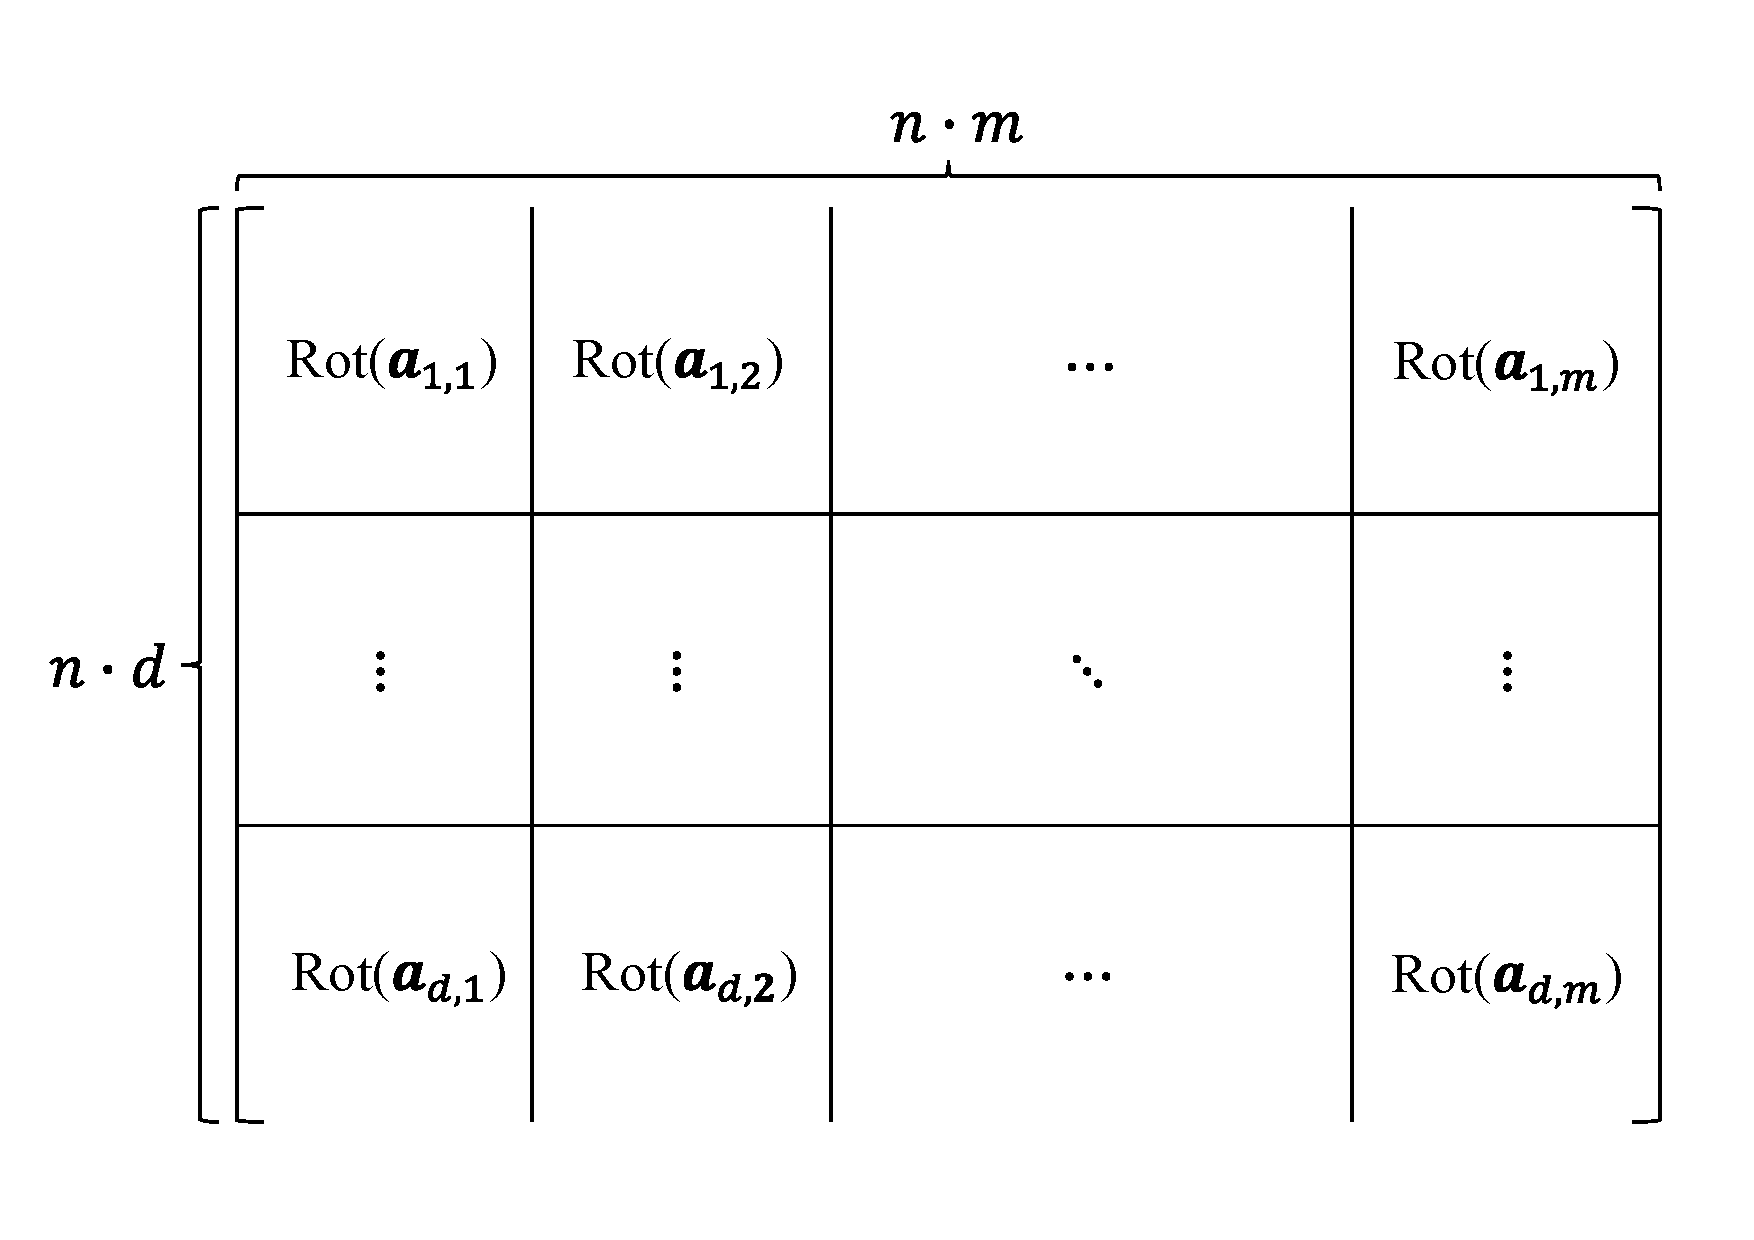
\includegraphics[width=0.7\textwidth]{graphics/MSIS_matrix.pdf}
\end{center}
An MSIS$_{n, d, q, m, \beta}$ instance thus becomes an SIS$_{n\cdot d, q, m \cdot n, \beta}$ instance.


For LWE, we will only list the definition of the ring and module variant. We are aware that we have not introduced the underlying math and refer the reader to \cite{LS15}. Let us just note here that $\mathcal{R}^\perp$ refers to the dual of $\mathcal{R}$.
\begin{definition}[Ring-LWE (RLWE) Distribution \cite{LS15}]
    Let $\chi$ be the error distribution on $\mathbb{T}_{\mathcal{R}^\perp} = K_\mathbb{R} / \mathcal{R}^\perp$ and $s \in \mathcal{R}^\perp$ be the secret. Then, we define $\mathcal{A}_{q, s, \chi}^{(\mathcal{R})}$ as the RLWE distribution on $\mathcal{R}_q \times \mathbb{T}_{\mathcal{R}^\perp}$ obtained by choosing $a \in \mathbb{R}_q$ uniformly at random and an error term $e \in \mathbb{T}_{\mathcal{R}^\perp}$ according to $\chi$, and returning samples $(a, (a \cdot s)/q + e)$.
\end{definition}

The search version of RLWE$_{n, q, m, \chi}$ asks us to find $s$ given $m$ samples from $\mathcal{A}_{q, s, \chi}^{(\mathcal{R})}$ with modulus $q\geq 2$ and $n$ the degree of the polynomial of $\mathcal{R}$. The decision version asks us to distinguish between $m$ samples from $\mathcal{A}_{q, s, \chi}^{(\mathcal{R})}$ and $m$ independent samples from the uniform distribution over $\mathcal{R}_q \times \mathbb{T}_{\mathcal{R}^\perp}$.

\begin{definition}[Module-LWE (MLWE) Distribution \cite{LS15}]
    Let $\chi$ be the error distribution on $\mathbb{T}_{\mathcal{R}^\perp}$ and $\mathbf{s} \in (\mathcal{R}^\perp)^d$ be the secret vector. Then, we define $\mathcal{A}_{q, \mathbf{s}, \chi}^{(\mathcal{M})}$ as the MLWE distribution on $(\mathcal{R}_q)^d \times \mathbb{T}_{\mathcal{R}^\perp}$ obtained by choosing $\mathbf{a} \in (\mathbb{R}_q)^d$ uniformly at random and an error term $e \in \mathbb{T}_{\mathcal{R}^\perp}$ according to $\chi$, and returning samples $(\mathbf{a}, \frac{1}{q}\langle \mathbf{a},\mathbf{s}\rangle + e)$.
\end{definition}

Analogously, the search version of MLWE$_{n, d, q, m, \chi}$ asks us to find $\mathbf{s}$ given $m$ samples from $\mathcal{A}_{q, \mathbf{s}, \chi}^{(\mathcal{M})}$ with modulus $q\geq 2$, $n$ the degree of the polynomial of $\mathcal{R}$ and modulus rank $d$. The decision version asks us to distinguish between $m$ samples from $\mathcal{A}_{q, \mathbf{s}, \chi}^{(\mathcal{M})}$ and $m$ independent samples from the uniform distribution over $\mathcal{R}_q^d \times \mathbb{T}_{\mathcal{R}^\perp}$.

We can construct a matrix $\mathbf{A}$ of the $a_i$ of RLWE and $\mathbf{a}_i$ of MLWE, as for standard LWE, to formulate the problems as a decoding problem, as in \cref{sec:lwe-decoding}. We interpret RLWE$_{n, q, m, \chi}$ and MLWE$_{n, d, q, m, \chi}$ as instances of LWE$_{n, q, m \cdot d, \chi'}$ and RLWE$_{n\cdot d, q, m \cdot n, \chi'}$ respectively. For a summary of our results, see \cref{sec:problem-classes}.

